\documentclass[11pt]{article}

\usepackage{amsmath}
\usepackage{enumitem}
\usepackage{commath}
\usepackage{tikz}
\usetikzlibrary{calc}
\usepackage{cancel}
\usepackage{subfigure}
\usepackage{multicol}

\usepackage{graphicx}
\graphicspath{{images/}}

\usepackage{my_notes}
\usepackage{my_math}

\newenvironment{mybox}
{\begin{tcolorbox}[colback=red!5!white,colframe=red!75!black]}
{\end{tcolorbox}}

\newtheorem{proof}{Proof}

\newenvironment{mytbox}
{\begin{tcolorbox}[colback=red!5!white,colframe=red!75!black,title=test]}
{\end{tcolorbox}}

\begin{document}
%learn MATPLOTLIB!!!!
\title{Calc III Notes}
\author{Sean Richardson}
\date{\today}
\maketitle
%\tableofcontents

\section{2D and 3D Space}
\subsection{Cartesian Coordinates}
\subsection{Contour Maps}
\subsection{Quadratic Surfaces}
A quadratic surface is any combination of $x$'s, $y$'s, and $z$'s of orders $0$, $1$, or $2$. Here are some simple combinations of these:
\begin{equation*}
    R^2 = x^2 + y^2 + z^2
    \tag{Sphere}
\end{equation*}
The above equation holds for every $(x,y,z)$ coordinate that is a distance $R$ from the origin. So, this expresses a sphere of radius $R$.
\begin{equation*}
    R^2 = {(ax)}^2 = {(by)}^2 + {(cz)}^2
    \tag{Ellipsoid}
\end{equation*}
The added constants squishes the sphere by a factor of $a$ in the $x$ direction, $b$ in the $y$ direction, and $c$ in the $z$ direction resulting in an ellipsoid.

\begin{equation*}
    z = x^2+y^2
    \tag{Paraboloid}
\end{equation*}
The 2D equation $R^2 = x^2+y^2$ traces out a circle of radius $R$. Equivalently, the above equation traces out a circle of radius $\sqrt{z}$ at each $z$, resulting in a bowl; specifically, a ``Paraboloid''.
\marginpar{Add Picture[s]}
\begin{equation*}
    z = x^2-y^2
    \tag{Saddle}
\end{equation*}
The 2D equation $A = x^2 - y^2$
\begin{equation*}
    z = xy
    \tag{Saddle}
\end{equation*}
\marginpar{Finish up}
The last three quadratic surfaces have the form of $z = ax^2+bxy+cy^2$. These will either be a bowl or a saddle, which you can determine with the following rule.
\begin{mybox}
For equations of the form,
\begin{equation*}
   z = ax^2+bxy+cy^2
\end{equation*}
Consider the quantity $Q = b^2-4ac$. The quadratic is a saddle if $Q > 0$, a bowl if $Q < 0$ and a taco if $Q = 0$.
\end{mybox}
\begin{proof}
Do this!
\end{proof}
co\marginpar{explain `taco'}
\subsection{Vectors and Matrices}
\marginpar{LA reference}
\subsection{Vector Fields}
\subsection{Parallelogram Grid}
\subsection{Transformations}
Previous math classes have addressed simple functions that take $1$ variable as an input and $1$ variable as an output. We visualized these functions through graphs, where one dimension (the $x$ axis) is reserved for inputs and one direction (the $y$ axis) is reserved for outputs. Functions with two inputs and one output you learned as three dimensional functions --- the $x$ and $y$ axes are inputs and the $z$ axis is the output. However, once we reach $2$ inputs, $(u,v)$, and $2$ outputs, $(x,y)$, we have run out of dimensions to visualize in. The idea of a \textit{transformation} is an alternate visualization technique that instead transforms the input $(u,v)$ plane into the output $(x,y)$ plane. The transformation simply demonstrates how grid lines in the input space are distorted into the output space.
\marginpar{transformation example figure}
\subsection{Dot Product}
The dot product is an operation that takes two vectors as inputs and outputs a scalar.
\begin{mybox}
    For two vectors $\vec{a}=\myvec{a_x,a_y}$ and $\vec{b}=\myvec{b_x,b_y}$, the dot product is denoted $\vec{a} \cdot \vec{b}$ and is equivalent to:
    \begin{equation*}
        \vec{a} \cdot \vec{b} = \mymag{\vec{a}}\mymag{\vec{b}}\cos{\theta} = a_x b_x+a_y b_y
    \end{equation*}
    Where $\theta$ is the angle between the two vectors.\\
    In $n$ dimensions, for $a = \myvec{a_1,a_2,\ldots,a_n}$ and $b = \myvec{b_1,b_2,\ldots,b_n}$
    \begin{equation*}
    \vec{a} \cdot \vec{b} = \mymag{\vec{a}}\mymag{\vec{b}}\cos{\theta} = \sum_i a_i b_i
    \end{equation*}
\end{mybox}
\begin{proof}
    The derivation of the dot product is related to the law of cosines. Consider the left triangle shown in Figure~\ref{two_triangles}.
\begin{figure}
\centering
\begin{subfigure}
    \centering
    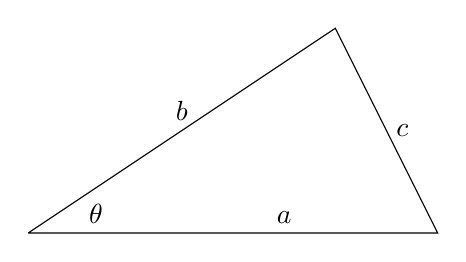
\begin{tikzpicture}[scale=1.3]
				%\draw [help lines] (0,0) grid (4,2);
				\draw (0,0) -- (3,2) -- (4,0) -- (0,0);
				\node [above right] at (0.5,0) {$\theta$};
				\node [above] at (1.5,1) {$b$};
				\node [right] at (3.5,1) {$c$};
				\node [above] at (2.5,0) {$a$};
	\end{tikzpicture}
\end{subfigure}
			%Law of cosines figure -- vector addition
\begin{subfigure}
    \centering
    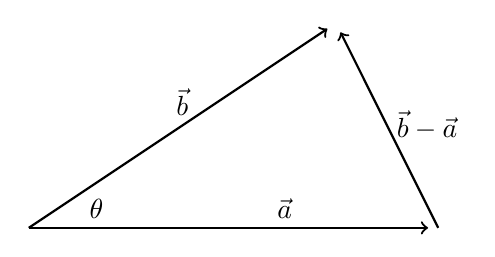
\begin{tikzpicture}[scale=1.3]
        \coordinate (A) at (0,0);
        \coordinate (B) at (3,2);
        \coordinate (C) at (4,0);
        \draw [thick, ->] (A) -- ($ (B)!0.1cm!(A) $);
        \draw [thick, ->] (4,0) -- ($ (B)!0.1cm!(C) $);
        \draw [thick, ->] (0,0) -- ($ (C)!0.1cm!(A)$);
        \node [above right] at (0.5,0) {$\theta$};
        \node [above] at (1.5,1) {$\vec b$};
        \node [right] at (3.5,1) {$\vec b - \vec a$};
        \node [above] at (2.5,0) {$\vec a$};
    \end{tikzpicture}
\end{subfigure}
\caption{Law of Cosines through Vectors}
\label{two_triangles}
\end{figure}
According to the law of cosines,
\begin{equation*}
    c^2=a^2+b^2-2ab\cos{\theta}
\end{equation*}
Where $a$, $b$, and $c$ refer to the length of each side of the triangle. Equivalently, we can express lengths as the magnitudes of the vectors shown on the right triangle of Figure \ref{two_triangles}.
\begin{equation*}
    \mymag{\vec{b}-\vec{a}}^2=\mymag{\vec{a}}^2+\mymag{\vec{b}}^2-2\mymag{\vec{a}}\mymag{\vec{b}}\cos{\theta}
\end{equation*}
Using the distance formula, we expand the expressions for the magnitudes of each vector.
\begin{align*}
    (b_x-a_x)^2 + (b_y-a_y)^2 &= a_x^2 + a_y^2 + b_x^2 + b_y^2 - 2\mymag{\vec a}\mymag{\vec b}\cos{\theta}\\
    \cancel{b_x^2}-2a_xb_x+\cancel{a_x^2}+\cancel{b_y^2}-2a_yb_y+\cancel{a_y^2}	&= \cancel{a_x^2} + \cancel{a_y^2} + \cancel{b_x^2} + \cancel{b_y^2} - 2\mymag{\vec a}\mymag{\vec b}\cos{\theta}\\
    a_xb_x+a_yb_y &= \mymag{\vec a}\mymag{\vec b}\cos{\theta}
\end{align*}
The above equality turns out to be useful and often used. So, we name each side of the equality the ``dot product'' and denote it as $\vec{a} \cdot \vec{b}$. While the above proof is specific to two dimensional vectors, it generalizes to $n$ dimensions.
\end{proof}
\subsection{Cross Product}
In three dimensional space, vectors have a unique property. Given two vectors, there is a single direction that is orthogonal to both initial vectors. It is often useful to find this direction, which we do so through a tool called the ``cross product''. The cross product takes in two vectors and outputs a vector in the orthogonal direction.
\begin{mybox}
    For two vectors $\vec{a}=\myvec{a_x,a_y,a_z}$ and $\vec{b}=\myvec{b_x,b_y,b_z}$, the cross product is denoted $\vec{a} \times \vec{b}$ and is equivalent to:
    \begin{equation*}
        \vec{a} \times \vec{b} = \myvec{a_yb_z-a_zb_y,a_zb_x-a_xb_z,a_xb_y-a_yb_x}
    \end{equation*}
    The resulting vector, $\vec{a} \times \vec{b}$, will be orthogonal to both $\vec{a}$ and $\vec{b}$.
\end{mybox}
\begin{proof}
    The claim is that $\vec{a} \times \vec{b}$ is orthogonal to $\vec{a}$ and $\vec{b}$. If the dot products between $\vec{a} \times \vec{b}$ and the two vectors is $0$, then we will have shown orthogonality. First, we evaluate $\vec{a} \cdot (\vec{a}\times\vec{b})$,
    \begin{align*}
        \vec{a} &\cdot (\vec{a}\times\vec{b})\\
        \myvec{a_x,a_y,a_z} &\cdot \myvec{a_yb_z-a_zb_y,a_zb_x-a_xb_z,a_xb_y-a_yb_x}
    \end{align*}
    Now, we cary out the dot product,
    \begin{equation*}
        a_xa_yb_z-a_xa_zb_y+a_ya_zb_x-a_xa_yb_z+a_xa_zb_y-a_ya_zb_x
    \end{equation*}
    Every term has a partner of opposite sign to cancel with, so the dot product evaluates to $0$. Therefore, $\vec{a}\times\vec{b}$ is orthogonal to $\vec{a}$. The same argument is applied to $\vec{b}$.
\begin{align*}
        \vec{b} &\cdot (\vec{a}\times\vec{b})\\
        \myvec{b_x,b_y,b_z} &\cdot \myvec{a_yb_z-a_zb_y,a_zb_x-a_xb_z,a_xb_y-a_yb_x}\\
        a_yb_xb_y-a_zb_xb_y&+a_zb_xb_y-a_xb_yb_z+a_xb_xb_y-a_yb_xb_z=0
\end{align*}
And therefore, the cross product $\vec{a}\times\vec{b}$ does indeed output a vector orthogonal to both $\vec{a}$ and $\vec{b}$.
\end{proof}
\marginpar{Cross product properties and techniques}
\section{???}
\subsection{Curvilinear Coordinization}
\subsubsection{Polar Coordinates}
In 2D space, we typically communicate the location of a point with $(x,y)$ coordinates; however, there are other ways. One such way is to use ``polar coordinates''. Consider a vector going from the origin to an unknown point. If we knew the length and direction of this vector, we could find the point. In polar coordinates, we denote the length of this vector with $r$. The direction is communicated with $\theta$, the angle the vector makes with the positive $x$ axis. Polar coordinates are $(r,\theta)$ pairs that specify a point.
\marginpar{Add figures}
%\begin{tikzpicture}
%    \coordinate (O) at (0,0);
%    \coordinate (A) at (4,0);
%    \coordinate (B) at (4,2);
%    \draw[helpines] (0,0) grid (5,5);
%    \draw[thick, ->] (O) -- (5,0);
%    \draw[thick, ->] (O) -- (0,3);
%    \draw[blue] (O) -- (A);
%    \draw[blue] (A) -- (B);
%    \draw[red] (O) -- (B); 
%\end{tikzpicture}
%\begin{tikzpicture}
%    \draw[helplines] (0:0) grid (5:3);
%\end{tikzpicture}
Using simple trigonometry, we can relate polar coordinates to cartesian coordinates. 
\begin{mybox}
    Translating between polar $(r,\theta)$ and cartesian $(x,y)$ coordinates.
    \begin{align*}
        \begin{split}
        x &= r\cos{\theta}\\
        y &= r\sin{\theta}
        \end{split}
        \begin{split}
        r &= \sqrt{x^2+y^2} \\
        \theta &= \arctan{\left(y/x\right)} [+\pi?]
        \end{split}
    \end{align*}
    In calculating $\theta$, you must add $\pi$ if $(x,y)$ is in quadrants $3$ or $4$.
\end{mybox}
\subsubsection{Cylindrical Coordinates}
\begin{mybox}
    Translating between cylindrical $(r_{cyl},\theta,z)$ and cartesian $(x,y,z)$ coordinates.
    \begin{align*}
        \begin{split}
            x &= r_{cyl}\cos{\theta}\\
            y &= r_{cyl}\sin{\theta}\\
            z &= z
        \end{split}
        \begin{split}
            r_{cyl} &= \sqrt{x^2+y^2} \\
        \theta &= \arctan{\left(y/x\right)} [+\pi?]\\
        z &= z
        \end{split}
    \end{align*}
    In calculating $\theta$, you must add $\pi$ if the point is in quadrants $3$ or $4$.
\end{mybox}
\subsubsection{Spherical Coordinates}
\begin{mybox}
Translating between spherical $(r_{sph},\theta,\phi)$ and cartesian $(x,y,z)$ coordinates.
    \begin{align*}
        \begin{split}
            x &= r_{sph}\cos{\theta}\sin{\phi}\\
            y &= r_{sph}\sin{\theta}\sin{\phi}\\
            z &= r_{sph}\cos{\phi}
        \end{split}
        \begin{split}
            r_{sph} &= \sqrt{x^2+y^2+z^2}\\
            \theta  &= \arctan{\left(y/x\right)} [+\pi?]\\
            \phi    &= \arccos{\left(\frac{z}{\sqrt{x^2+y^2+z^2}}\right)}
        \end{split}
    \end{align*}
    In calculating $\theta$, you must add $\pi$ if the point is in quadrants $3$ or $4$.
\end{mybox}

\subsection{Coordinate Vector Fields}
Consider a mapping from curvilinear space to cartesian space. Coordinate vector fields have the job of pointing in the direction curviliear values increase within cartesian space.
\begin{mybox}
    Consider some transformation $T(u,v)=(x,y)$. The direction and magnitude in which an arbitrary curvilinear coordinate, $u$, increases at any given $(u,v)$ is given by the coordinate vector field, $\partial_u = \myvec{\mypder{x}{u},\mypder{y}{u}}$.
\end{mybox}
\marginpar{justification?}
\subsubsection{Polar Vector Field}
For the polar coordinate transformation, $(x,y)=T(r,\theta)=(r\cos{\theta},r\sin{\theta})$, we are interested in finding the direction of increase of 
\subsubsection{Cylindrical Vector Field}
\subsubsection{Spherical Vector Field}
\subsection{Linearization}
Take some curvilinear transformation $(x,y) = T(u,v)$. This is a mapping of straight gridlines into bent gridlines. However, if we zoom into the output space enough, the gridlines will begin to appear as straight. The directions of these gridlines are given by the partial vectors, $\partial_u$ and $\partial_v$, at that point. So, the gridlines are close to straight, we can approximate a short journey along the $u,v$ gridlines in the $x,y$ plane by following the direction of the partial vectors, $\partial_u$ and $\partial_v$.\\
Following the $u,v$ gridlines by small amounts $\Delta u$ and $\Delta v$ results in the following changes in $x$ and $y$:
\begin{align*}
    \begin{split}
        &\text{Effect of following $u$ gridline:}\\
        \begin{pmatrix} \Delta x \\ \Delta y \end{pmatrix}
        &\approx \partial_u \cdot \Delta u \\
        \begin{pmatrix} \Delta x \\ \Delta y \end{pmatrix}
        &\approx \mypder{x}{u}\Delta u + \mypder{y}{u}\Delta u
    \end{split}
    \begin{split}
        &\text{Effect of following $v$ gridline:}\\
        \begin{pmatrix} \Delta x \\ \Delta y \end{pmatrix}
        &\approx \partial_u \cdot \Delta u \\
        \begin{pmatrix} \Delta x \\ \Delta y \end{pmatrix}
        &\approx \mypder{x}{u}\Delta u + \mypder{y}{u}\Delta u
    \end{split}
\end{align*}
Combining the effects of traveling along the two gridlines through addition gives the following.
\begin{align*}
    \begin{pmatrix} \Delta x \\ \Delta y \end{pmatrix}
    &\approx \mypder{x}{u}\Delta u + \mypder{y}{u}\Delta u
    + \mypder{x}{v}\Delta v + \mypder{y}{v}\Delta v
\end{align*}
We now condense this expression with matrix notation.
\begin{equation}
    \begin{pmatrix} \Delta x \\ \Delta y \end{pmatrix}
    \approx \begin{pmatrix}
    \mypder{x}{u} && \mypder{x}{v} \\[6pt]
    \mypder{y}{v} && \mypder{y}{v}
    \end{pmatrix}
    \begin{pmatrix} \Delta u \\ \Delta v \end{pmatrix}
    \label{eq:linearization}
\end{equation}
This equation approximates how movement in the input $u,v$ plane translates to movement in the output $x,y$ plane. The matrix appearing in the above equation is widely used, so it gets the name ``Jacobian matrix''.
\begin{mybox}
    The \textit{Jacobian Matrix} of a transformation $T$ is abreviated as $DT$ and consits of the partial vectors of the transformation in each column. For the transformation $(x,y) = T(u,v)$:
        $DT = \begin{pmatrix}
        \mypder{x}{u} && \mypder{x}{v} \\[6pt]
        \mypder{y}{v} && \mypder{y}{v}
    \end{pmatrix}$.
    In general, the Jacobian Matrix for a transformation $(x^1,x^2,\ldots,x^n) = T(y^1,y^2,\ldots,y^m)$ is given by,
    \begin{equation*}
    DT = \begin{pmatrix}
        \mypder{x^1}{y^1} & \cdots & \mypder{x^1}{y^m} \\
        \vdots            & \ddots& \vdots\\
        \mypder{x^n}{y^1} & \cdots & \mypder{x^n}{y^m}
    \end{pmatrix}
    \text{Where the $(i,j)$ entry of $DT$ is $DT_{ij} = \mypder{x^i}{y^j}$}
    \end{equation*}
\end{mybox}
\noindent We can now combine equation~\ref{eq:linearization} with the idea of a Jacobian Matrix to formally introduce linearization.
\begin{mybox}
    Given a transformation $(x,y)=T(u,v)$, the \textit{linearization} is the linear approximation of how a small change in $u$ and $v$ affects $x$ and $y$ given by the following equation,
\begin{equation*}
\begin{pmatrix} \Delta x \\ \Delta y \end{pmatrix}
    \approx DT
    \begin{pmatrix} \Delta u \\ \Delta v \end{pmatrix}
\end{equation*}
    In general, for $(x^1,x^2,\ldots,x^n) = T(y^1,y^2,\ldots,y^m)$:
\begin{equation*}
    \begin{pmatrix} \Delta x^1 \\ \vdots \\ \Delta x^n \end{pmatrix}
    \approx DT
    \begin{pmatrix} \Delta y^1 \\ \vdots \\ \Delta y^m \end{pmatrix}
\end{equation*}
\end{mybox}
\marginpar{error analysis}
\subsection{Chain Rule}

\end{document}
